\subsection{VSD: Visible Surface Determination}
To determine what is visible and draw things properly is hard. Michael Abrash summarized the domain of the problem well:\\

\begin{fancyquotes}
I want to talk about what is, in my book, the toughest 3-D problem of all, visible surface determination (drawing the proper surface at each pixel), and its close relative, culling (discarding non-visible polygons as quickly as possible, a way of accelerating visible surface determination). In the interests of brevity, I’ll use the abbreviation VSD to mean both visible surface determination and culling from now on.
 \bigskip \\
Why do I think VSD is the toughest 3-D challenge? Although rasterization issues such as texture mapping are fascinating and important, they are tasks of relatively finite scope, and are being moved into hardware as 3-D accelerators appear; also, they only scale with increases in screen resolution, which are relatively modest.
 \bigskip \\
In contrast, VSD is an open-ended problem, and there are dozens of approaches currently in use. Even more significantly, the performance of VSD, done in an unsophisticated fashion, scales directly with scene complexity, which tends to increase as a square or cube function, so this very rapidly becomes the limiting factor in doing realistic worlds. I expect VSD increasingly to be the dominant issue in realtime PC 3-D over the next few years, as 3-D worlds become increasingly detailed.
 \bigskip \\
\bigskip \\
\textbf{Michael Abrash - Programmer}
 \end{fancyquotes}
 
 Wolf3D uses two mechanism to make sure things are draw properly:
 \begin{enumerate}
 	\item While casting each ray, memorize which cells were visited by the ray. This is used to know which "things" to draw.
 	\item Upon drawing a wall column, save the height of that wall. This is done to clip "things" to draw.
 \end{enumerate}
 
 \subsubsection{}
 At the beginning of each 3D rendition, the engine clears the:
 \lstinputlisting[language=C]{code/clear_vis_wold3d.c}
 Note that because register are 2 bytes wide, an array of 64x64=4096 bytes can be zeroed in 2048 iterations. Nowadays it is more efficient to use the C library.
 \lstinputlisting[language=C]{code/clear_vis_modern.c}
 Later in the assembly hand crafted procedure \codeword{AsmRefresh} we can find where this array is populated:
  \lstinputlisting[language={[x86masm]Assembler}]{code/mark_vis_wold3d.asm}
  If we take the example of the starting screen, we can see which tile were marked at visible:
  
  
\begin{figure}[H]
  \centering
  
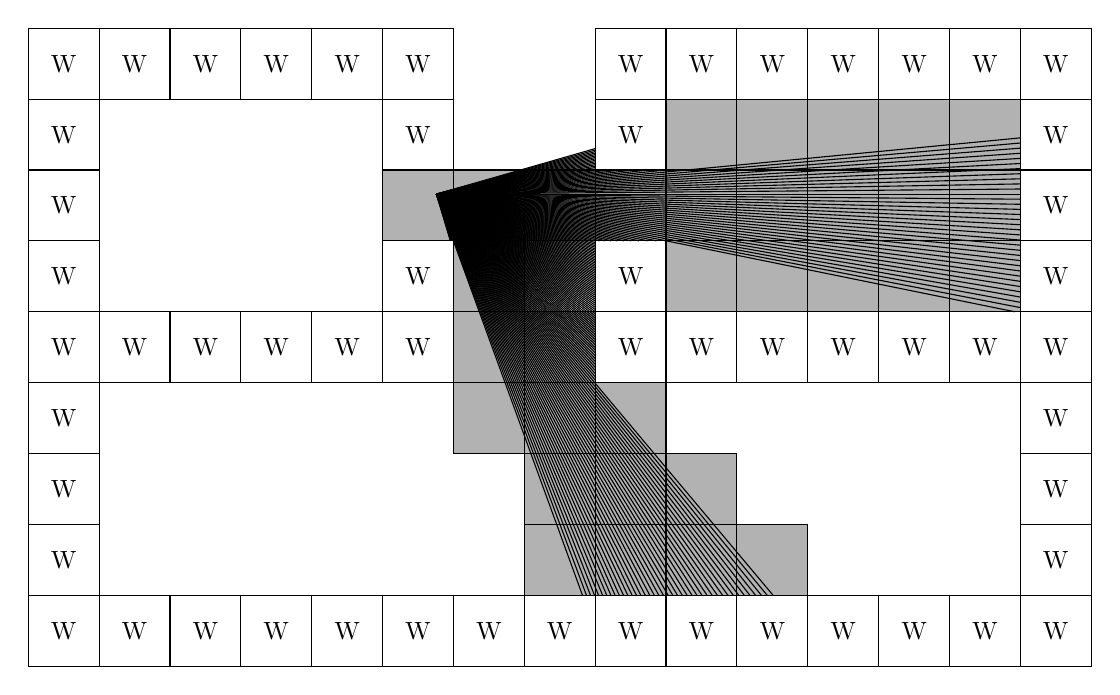
\begin{tikzpicture}[y=-1cm,scale=0.9, every node/.style={scale=0.9}]


\draw (27,55) rectangle (28,56) node[pos=.5] {W};
\draw (27,56) rectangle (28,57) node[pos=.5] {W};
\draw (27,57) rectangle (28,58) node[pos=.5] {W};
\draw (27,58) rectangle (28,59) node[pos=.5] {W};
\draw (27,59) rectangle (28,60) node[pos=.5] {W};
\draw (27,60) rectangle (28,61) node[pos=.5] {W};
\draw (27,61) rectangle (28,62) node[pos=.5] {W};
\draw (27,62) rectangle (28,63) node[pos=.5] {W};
\draw (27,63) rectangle (28,64) node[pos=.5] {W};
\draw (28,55) rectangle (29,56) node[pos=.5] {W};
\draw (28,59) rectangle (29,60) node[pos=.5] {W};
\draw (28,63) rectangle (29,64) node[pos=.5] {W};
\draw (29,55) rectangle (30,56) node[pos=.5] {W};
\draw (29,59) rectangle (30,60) node[pos=.5] {W};
\draw (29,63) rectangle (30,64) node[pos=.5] {W};
\draw (30,55) rectangle (31,56) node[pos=.5] {W};
\draw (30,59) rectangle (31,60) node[pos=.5] {W};
\draw (30,63) rectangle (31,64) node[pos=.5] {W};
\draw (31,55) rectangle (32,56) node[pos=.5] {W};
\draw (31,59) rectangle (32,60) node[pos=.5] {W};
\draw (31,63) rectangle (32,64) node[pos=.5] {W};
\draw (32,55) rectangle (33,56) node[pos=.5] {W};
\draw (32,56) rectangle (33,57) node[pos=.5] {W};
\draw (32,58) rectangle (33,59) node[pos=.5] {W};
\draw (32,59) rectangle (33,60) node[pos=.5] {W};
\draw (32,63) rectangle (33,64) node[pos=.5] {W};
\draw (33,63) rectangle (34,64) node[pos=.5] {W};
\draw (34,63) rectangle (35,64) node[pos=.5] {W};
\draw (35,55) rectangle (36,56) node[pos=.5] {W};
\draw (35,56) rectangle (36,57) node[pos=.5] {W};
\draw (35,58) rectangle (36,59) node[pos=.5] {W};
\draw (35,59) rectangle (36,60) node[pos=.5] {W};
\draw (35,63) rectangle (36,64) node[pos=.5] {W};
\draw (36,55) rectangle (37,56) node[pos=.5] {W};
\draw (36,59) rectangle (37,60) node[pos=.5] {W};
\draw (36,63) rectangle (37,64) node[pos=.5] {W};
\draw (37,55) rectangle (38,56) node[pos=.5] {W};
\draw (37,59) rectangle (38,60) node[pos=.5] {W};
\draw (37,63) rectangle (38,64) node[pos=.5] {W};
\draw (38,55) rectangle (39,56) node[pos=.5] {W};
\draw (38,59) rectangle (39,60) node[pos=.5] {W};
\draw (38,63) rectangle (39,64) node[pos=.5] {W};
\draw (39,55) rectangle (40,56) node[pos=.5] {W};
\draw (39,59) rectangle (40,60) node[pos=.5] {W};
\draw (39,63) rectangle (40,64) node[pos=.5] {W};
\draw (40,55) rectangle (41,56) node[pos=.5] {W};
\draw (40,59) rectangle (41,60) node[pos=.5] {W};
\draw (40,63) rectangle (41,64) node[pos=.5] {W};
\draw (41,55) rectangle (42,56) node[pos=.5] {W};
\draw (41,56) rectangle (42,57) node[pos=.5] {W};
\draw (41,57) rectangle (42,58) node[pos=.5] {W};
\draw (41,58) rectangle (42,59) node[pos=.5] {W};
\draw (41,59) rectangle (42,60) node[pos=.5] {W};
\draw (41,60) rectangle (42,61) node[pos=.5] {W};
\draw (41,61) rectangle (42,62) node[pos=.5] {W};
\draw (41,62) rectangle (42,63) node[pos=.5] {W};
\draw (41,63) rectangle (42,64) node[pos=.5] {W};

\filldraw[fill=black!30!white, draw=black] (32,57) rectangle (33,58);
\filldraw[fill=black!30!white, draw=black] (33,57) rectangle (34,58);
\filldraw[fill=black!30!white, draw=black] (34,57) rectangle (35,58);
\filldraw[fill=black!30!white, draw=black] (35,57) rectangle (36,58);

% Room
\filldraw[fill=black!30!white, draw=black] (36,57) rectangle (37,58);
\filldraw[fill=black!30!white, draw=black] (37,57) rectangle (38,58);
\filldraw[fill=black!30!white, draw=black] (38,57) rectangle (39,58);
\filldraw[fill=black!30!white, draw=black] (39,57) rectangle (40,58);
\filldraw[fill=black!30!white, draw=black] (40,57) rectangle (41,58);

\filldraw[fill=black!30!white, draw=black] (36,58) rectangle (37,59);
\filldraw[fill=black!30!white, draw=black] (37,58) rectangle (38,59);
\filldraw[fill=black!30!white, draw=black] (38,58) rectangle (39,59);
\filldraw[fill=black!30!white, draw=black] (39,58) rectangle (40,59);
\filldraw[fill=black!30!white, draw=black] (40,58) rectangle (41,59);

\filldraw[fill=black!30!white, draw=black] (36,56) rectangle (37,57);
\filldraw[fill=black!30!white, draw=black] (37,56) rectangle (38,57);
\filldraw[fill=black!30!white, draw=black] (38,56) rectangle (39,57);
\filldraw[fill=black!30!white, draw=black] (39,56) rectangle (40,57);
\filldraw[fill=black!30!white, draw=black] (40,56) rectangle (41,57);


\filldraw[fill=black!30!white, draw=black] (33,58) rectangle (34,59);
\filldraw[fill=black!30!white, draw=black] (33,59) rectangle (34,60);
\filldraw[fill=black!30!white, draw=black] (33,60) rectangle (34,61);
%\filldraw[fill=black!30!white, draw=black] (33,61) rectangle (34,62);
%\filldraw[fill=black!30!white, draw=black] (33,62) rectangle (34,63);
%\filldraw[fill=black!30!white, draw=black] (34,58) rectangle (35,59);
\filldraw[fill=black!30!white, draw=black] (34,59) rectangle (35,60);
\filldraw[fill=black!30!white, draw=black] (34,60) rectangle (35,61);
\filldraw[fill=black!30!white, draw=black] (34,61) rectangle (35,62);
\filldraw[fill=black!30!white, draw=black] (34,62) rectangle (35,63);

% Triangle
\filldraw[fill=black!30!white, draw=black] (35,60) rectangle (36,61);

\filldraw[fill=black!30!white, draw=black] (35,61) rectangle (36,62);
\filldraw[fill=black!30!white, draw=black] (36,61) rectangle (37,62);

\filldraw[fill=black!30!white, draw=black] (35,62) rectangle (36,63);
\filldraw[fill=black!30!white, draw=black] (36,62) rectangle (37,63);
\filldraw[fill=black!30!white, draw=black] (37,62) rectangle (38,63);

\draw[thin,black] (32.759998,57.340000) -- (35.000000,56.697712);
\draw[thin,black] (32.759998,57.340000) -- (35.000000,56.718815);
\draw[thin,black] (32.759998,57.340000) -- (35.000000,56.739815);
\draw[thin,black] (32.759998,57.340000) -- (35.000000,56.760712);
\draw[thin,black] (32.759998,57.340000) -- (35.000000,56.781525);
\draw[thin,black] (32.759998,57.340000) -- (35.000000,56.802242);
\draw[thin,black] (32.759998,57.340000) -- (35.000000,56.822868);
\draw[thin,black] (32.759998,57.340000) -- (35.000000,56.843414);
\draw[thin,black] (32.759998,57.340000) -- (35.000000,56.863884);
\draw[thin,black] (32.759998,57.340000) -- (35.000000,56.884285);
\draw[thin,black] (32.759998,57.340000) -- (35.000000,56.904602);
\draw[thin,black] (32.759998,57.340000) -- (35.000000,56.924854);
\draw[thin,black] (32.759998,57.340000) -- (35.000000,56.945038);
\draw[thin,black] (32.759998,57.340000) -- (35.000000,56.965164);
\draw[thin,black] (32.759998,57.340000) -- (35.000000,56.985229);
\draw[thin,black] (32.759998,57.340000) -- (35.035076,57.000000);
\draw[thin,black] (32.759998,57.340000) -- (35.179306,57.000000);
\draw[thin,black] (32.759998,57.340000) -- (35.342648,57.000000);
\draw[thin,black] (32.759998,57.340000) -- (35.529148,57.000000);
\draw[thin,black] (32.759998,57.340000) -- (35.744217,57.000000);
\draw[thin,black] (32.759998,57.340000) -- (35.994972,57.000000);
\draw[thin,black] (32.759998,57.340000) -- (41.000000,56.546600);
\draw[thin,black] (32.759998,57.340000) -- (41.000000,56.619114);
\draw[thin,black] (32.759998,57.340000) -- (41.000000,56.691517);
\draw[thin,black] (32.759998,57.340000) -- (41.000000,56.763821);
\draw[thin,black] (32.759998,57.340000) -- (41.000000,56.836033);
\draw[thin,black] (32.759998,57.340000) -- (41.000000,56.908173);
\draw[thin,black] (32.759998,57.340000) -- (41.000000,56.980244);
\draw[thin,black] (32.759998,57.340000) -- (41.000000,57.052261);
\draw[thin,black] (32.759998,57.340000) -- (41.000000,57.124237);
\draw[thin,black] (32.759998,57.340000) -- (41.000000,57.196175);
\draw[thin,black] (32.759998,57.340000) -- (41.000000,57.268093);
\draw[thin,black] (32.759998,57.340000) -- (41.000000,57.340000);
\draw[thin,black] (32.759998,57.340000) -- (41.000000,57.411907);
\draw[thin,black] (32.759998,57.340000) -- (41.000000,57.483826);
\draw[thin,black] (32.759998,57.340000) -- (41.000000,57.555763);
\draw[thin,black] (32.759998,57.340000) -- (41.000000,57.627739);
\draw[thin,black] (32.759998,57.340000) -- (41.000000,57.699757);
\draw[thin,black] (32.759998,57.340000) -- (41.000000,57.771828);
\draw[thin,black] (32.759998,57.340000) -- (41.000000,57.843967);
\draw[thin,black] (32.759998,57.340000) -- (41.000000,57.916180);
\draw[thin,black] (32.759998,57.340000) -- (41.000000,57.988483);
\draw[thin,black] (32.759998,57.340000) -- (41.000000,58.060886);
\draw[thin,black] (32.759998,57.340000) -- (41.000000,58.133400);
\draw[thin,black] (32.759998,57.340000) -- (41.000000,58.206036);
\draw[thin,black] (32.759998,57.340000) -- (41.000000,58.278805);
\draw[thin,black] (32.759998,57.340000) -- (41.000000,58.351715);
\draw[thin,black] (32.759998,57.340000) -- (41.000000,58.424782);
\draw[thin,black] (32.759998,57.340000) -- (41.000000,58.498020);
\draw[thin,black] (32.759998,57.340000) -- (41.000000,58.571438);
\draw[thin,black] (32.759998,57.340000) -- (41.000000,58.645050);
\draw[thin,black] (32.759998,57.340000) -- (41.000000,58.718861);
\draw[thin,black] (32.759998,57.340000) -- (41.000000,58.792892);
\draw[thin,black] (32.759998,57.340000) -- (41.000000,58.867146);
\draw[thin,black] (32.759998,57.340000) -- (41.000000,58.941647);
\draw[thin,black] (32.759998,57.340000) -- (40.919399,59.000000);
\draw[thin,black] (32.759998,57.340000) -- (35.865154,58.000000);
\draw[thin,black] (32.759998,57.340000) -- (35.737164,58.000000);
\draw[thin,black] (32.759998,57.340000) -- (35.618862,58.000000);
\draw[thin,black] (32.759998,57.340000) -- (35.509178,58.000000);
\draw[thin,black] (32.759998,57.340000) -- (35.407204,58.000000);
\draw[thin,black] (32.759998,57.340000) -- (35.312099,58.000000);
\draw[thin,black] (32.759998,57.340000) -- (35.223228,58.000000);
\draw[thin,black] (32.759998,57.340000) -- (35.139954,58.000000);
\draw[thin,black] (32.759998,57.340000) -- (35.061760,58.000000);
\draw[thin,black] (32.759998,57.340000) -- (35.000000,58.003498);
\draw[thin,black] (32.759998,57.340000) -- (35.000000,58.024818);
\draw[thin,black] (32.759998,57.340000) -- (35.000000,58.046249);
\draw[thin,black] (32.759998,57.340000) -- (35.000000,58.067799);
\draw[thin,black] (32.759998,57.340000) -- (35.000000,58.089470);
\draw[thin,black] (32.759998,57.340000) -- (35.000000,58.111271);
\draw[thin,black] (32.759998,57.340000) -- (35.000000,58.133202);
\draw[thin,black] (32.759998,57.340000) -- (35.000000,58.155266);
\draw[thin,black] (32.759998,57.340000) -- (35.000000,58.177475);
\draw[thin,black] (32.759998,57.340000) -- (35.000000,58.199829);
\draw[thin,black] (32.759998,57.340000) -- (35.000000,58.222332);
\draw[thin,black] (32.759998,57.340000) -- (35.000000,58.244991);
\draw[thin,black] (32.759998,57.340000) -- (35.000000,58.267807);
\draw[thin,black] (32.759998,57.340000) -- (35.000000,58.290791);
\draw[thin,black] (32.759998,57.340000) -- (35.000000,58.313950);
\draw[thin,black] (32.759998,57.340000) -- (35.000000,58.337280);
\draw[thin,black] (32.759998,57.340000) -- (35.000000,58.360794);
\draw[thin,black] (32.759998,57.340000) -- (35.000000,58.384499);
\draw[thin,black] (32.759998,57.340000) -- (35.000000,58.408390);
\draw[thin,black] (32.759998,57.340000) -- (35.000000,58.432484);
\draw[thin,black] (32.759998,57.340000) -- (35.000000,58.456787);
\draw[thin,black] (32.759998,57.340000) -- (35.000000,58.481300);
\draw[thin,black] (32.759998,57.340000) -- (35.000000,58.506027);
\draw[thin,black] (32.759998,57.340000) -- (35.000000,58.530987);
\draw[thin,black] (32.759998,57.340000) -- (35.000000,58.556183);
\draw[thin,black] (32.759998,57.340000) -- (35.000000,58.581608);
\draw[thin,black] (32.759998,57.340000) -- (35.000000,58.607285);
\draw[thin,black] (32.759998,57.340000) -- (35.000000,58.633221);
\draw[thin,black] (32.759998,57.340000) -- (35.000000,58.659416);
\draw[thin,black] (32.759998,57.340000) -- (35.000000,58.685879);
\draw[thin,black] (32.759998,57.340000) -- (35.000000,58.712627);
\draw[thin,black] (32.759998,57.340000) -- (35.000000,58.739658);
\draw[thin,black] (32.759998,57.340000) -- (35.000000,58.766991);
\draw[thin,black] (32.759998,57.340000) -- (35.000000,58.794624);
\draw[thin,black] (32.759998,57.340000) -- (35.000000,58.822567);
\draw[thin,black] (32.759998,57.340000) -- (35.000000,58.850845);
\draw[thin,black] (32.759998,57.340000) -- (35.000000,58.879452);
\draw[thin,black] (32.759998,57.340000) -- (35.000000,58.908405);
\draw[thin,black] (32.759998,57.340000) -- (35.000000,58.937721);
\draw[thin,black] (32.759998,57.340000) -- (35.000000,58.967392);
\draw[thin,black] (32.759998,57.340000) -- (35.000000,58.997452);
\draw[thin,black] (32.759998,57.340000) -- (35.000000,59.027897);
\draw[thin,black] (32.759998,57.340000) -- (35.000000,59.058746);
\draw[thin,black] (32.759998,57.340000) -- (35.000000,59.090012);
\draw[thin,black] (32.759998,57.340000) -- (35.000000,59.121704);
\draw[thin,black] (32.759998,57.340000) -- (35.000000,59.153843);
\draw[thin,black] (32.759998,57.340000) -- (35.000000,59.186440);
\draw[thin,black] (32.759998,57.340000) -- (35.000000,59.219505);
\draw[thin,black] (32.759998,57.340000) -- (35.000000,59.253059);
\draw[thin,black] (32.759998,57.340000) -- (35.000000,59.287125);
\draw[thin,black] (32.759998,57.340000) -- (35.000000,59.321701);
\draw[thin,black] (32.759998,57.340000) -- (35.000000,59.356819);
\draw[thin,black] (32.759998,57.340000) -- (35.000000,59.392494);
\draw[thin,black] (32.759998,57.340000) -- (35.000000,59.428741);
\draw[thin,black] (32.759998,57.340000) -- (35.000000,59.465588);
\draw[thin,black] (32.759998,57.340000) -- (35.000000,59.503048);
\draw[thin,black] (32.759998,57.340000) -- (35.000000,59.541145);
\draw[thin,black] (32.759998,57.340000) -- (35.000000,59.579899);
\draw[thin,black] (32.759998,57.340000) -- (35.000000,59.619339);
\draw[thin,black] (32.759998,57.340000) -- (35.000000,59.659481);
\draw[thin,black] (32.759998,57.340000) -- (35.000000,59.700356);
\draw[thin,black] (32.759998,57.340000) -- (35.000000,59.741989);
\draw[thin,black] (32.759998,57.340000) -- (35.000000,59.784412);
\draw[thin,black] (32.759998,57.340000) -- (35.000000,59.827652);
\draw[thin,black] (32.759998,57.340000) -- (35.000000,59.871735);
\draw[thin,black] (32.759998,57.340000) -- (35.000000,59.916695);
\draw[thin,black] (32.759998,57.340000) -- (35.000000,59.962570);
\draw[thin,black] (32.759998,57.340000) -- (37.509548,63.000000);
\draw[thin,black] (32.759998,57.340000) -- (37.425987,63.000000);
\draw[thin,black] (32.759998,57.340000) -- (37.343620,63.000000);
\draw[thin,black] (32.759998,57.340000) -- (37.262413,63.000000);
\draw[thin,black] (32.759998,57.340000) -- (37.182316,63.000000);
\draw[thin,black] (32.759998,57.340000) -- (37.103313,63.000000);
\draw[thin,black] (32.759998,57.340000) -- (37.025356,63.000000);
\draw[thin,black] (32.759998,57.340000) -- (36.948418,63.000000);
\draw[thin,black] (32.759998,57.340000) -- (36.872471,63.000000);
\draw[thin,black] (32.759998,57.340000) -- (36.797478,63.000000);
\draw[thin,black] (32.759998,57.340000) -- (36.723412,63.000000);
\draw[thin,black] (32.759998,57.340000) -- (36.650246,63.000000);
\draw[thin,black] (32.759998,57.340000) -- (36.577953,63.000000);
\draw[thin,black] (32.759998,57.340000) -- (36.506508,63.000000);
\draw[thin,black] (32.759998,57.340000) -- (36.435883,63.000000);
\draw[thin,black] (32.759998,57.340000) -- (36.366051,63.000000);
\draw[thin,black] (32.759998,57.340000) -- (36.296993,63.000000);
\draw[thin,black] (32.759998,57.340000) -- (36.228683,63.000000);
\draw[thin,black] (32.759998,57.340000) -- (36.161102,63.000000);
\draw[thin,black] (32.759998,57.340000) -- (36.094227,63.000000);
\draw[thin,black] (32.759998,57.340000) -- (36.028034,63.000000);
\draw[thin,black] (32.759998,57.340000) -- (35.962505,63.000000);
\draw[thin,black] (32.759998,57.340000) -- (35.897621,63.000000);
\draw[thin,black] (32.759998,57.340000) -- (35.833363,63.000000);
\draw[thin,black] (32.759998,57.340000) -- (35.769703,63.000000);
\draw[thin,black] (32.759998,57.340000) -- (35.706638,63.000000);
\draw[thin,black] (32.759998,57.340000) -- (35.644142,63.000000);
\draw[thin,black] (32.759998,57.340000) -- (35.582203,63.000000);
\draw[thin,black] (32.759998,57.340000) -- (35.520794,63.000000);
\draw[thin,black] (32.759998,57.340000) -- (35.459911,63.000000);
\draw[thin,black] (32.759998,57.340000) -- (35.399529,63.000000);
\draw[thin,black] (32.759998,57.340000) -- (35.339642,63.000000);
\draw[thin,black] (32.759998,57.340000) -- (35.280224,63.000000);
\draw[thin,black] (32.759998,57.340000) -- (35.221268,63.000000);
\draw[thin,black] (32.759998,57.340000) -- (35.162758,63.000000);
\draw[thin,black] (32.759998,57.340000) -- (35.104675,63.000000);
\draw[thin,black] (32.759998,57.340000) -- (35.047016,63.000000);
\draw[thin,black] (32.759998,57.340000) -- (34.989761,63.000000);
\draw[thin,black] (32.759998,57.340000) -- (34.932899,63.000000);
\draw[thin,black] (32.759998,57.340000) -- (34.876415,63.000000);
\draw[thin,black] (32.759998,57.340000) -- (34.820301,63.000000);
\draw[thin,black] (32.759998,57.340000) -- (32.993740,58.000000);
\draw[thin,black] (32.759998,57.340000) -- (32.987278,58.000000);
\draw[thin,black] (32.759998,57.340000) -- (32.980858,58.000000);
\draw[thin,black] (32.759998,57.340000) -- (32.974472,58.000000);
\draw[thin,black] (32.759998,57.340000) -- (32.968121,58.000000);
\draw[thin,black] (32.759998,57.340000) -- (32.961807,58.000000);
\draw[thin,black] (32.759998,57.340000) -- (32.955524,58.000000);
\end{tikzpicture}

 \caption{Ray cast and visible spots.} 
\end{figure}